\begin{exercise}{2016/17 5}
    \begin{enumerate}[label= (\alph*)]
        \item Μελετήστε το σύστημα στο επίπεδο
            \[
                \dot{x} = 2x - x^2, \quad \dot{y} = -y + xy.
            \]
            Βρείτε τα σημεία ισορροπίας, τον τύπο τους, καθώς και τις ευσταθείς
            και ασταθείς πολλαπλότητες καθενός από αυτά.

            Η \emph{θεωρία της δομικής ευστάθειας} λέει ότι, γενικά, κάθε ασταθής
            πολλαπλότητα ενός σημείου ισορροπίας (ή οριακού κύκλου) τέμνει την
            ευσταθή πολλαπλότητα άλλου σημείου ισορροπίας ή οριακού κύκλου
            \emph{εγκάρσια}.

            Δείξτε ότι στο παράδειγμα αυτό η τομή δεν είναι εγκάρσια. Είναι
            λοιπόν φυσικό να αναμένουμε ότι μικρές διαταραχές καταστρέφουν την
            μη-εγκάρσια αυτή τομή. Περιγράψτε τρόπους να γίνει αυτό.
            \emph{Υπόδειξη: επιλέξτε σημείο πάνω στην τροχιά που συνδέει τα
                σημεία ισορροπίας και με χρήση του κυτίου ροής (\tl{flow box})
            αλλάξτε τοπικά το διανυσματικό πεδίο}.
        \item Αναγνωρίστε παρόμοιες μη-εγκάρσιες τομές αναλλοίωτων πολλαπλοτήτων
            στις Χαμιλτονιανές περιπτώσεις των συστημάτων \tl{Duffing} και απλού
            εκκρεμούς.

            Συζητήστε κατά πόσο μπορούμε να φέρουμε τα συστήματα αυτά σε
            \enquote*{γενική θέση}, μένοντας όμως στην κατηγορία των
            Χαμιλτονιανών συστημάτων.
    \end{enumerate}
\end{exercise}
\begin{solution}{2016/17 5}
    (α). Τα σημεία ισορροπίας του συστήματος από την πρώτη σχέση είναι
    \begin{align*}
        0 &= 2x - x^2 \\
        0 &= x(2- x),
    \end{align*}
    άρα \( x = 0 \) ή \( x = 2 \). Από τη δεύτερη σχέση έχουμε
    \[
        0 = -y + xy.
    \]
    Άρα για \( x = 0 \) προκύπτει \( y = 0 \). Για \( x = 2 \) προκύπτει \( y =
    0 \). Ακόμα η δεύτερη εξίσωση μηδενίζεται για \( x = 1 \) και άρα εκεί το
    διανυσματικό πεδίο θα είναι παράλληλο το άξονα \( x \). Αν γράψουμε τις
    σχέσεις ως
    \[
        \begin{pmatrix}
            \dot{x} \\
            \dot{y}
        \end{pmatrix} = F(x, y)
        \begin{pmatrix}
            2x - x^2 \\
            -y + xy
            \dot{y}
        \end{pmatrix},
    \]
    τότε η γραμμικοποίηση είναι
    \[
        DF(x, y) =
        \begin{pmatrix}
            2 - 2x & 0 \\
            y & -1 + x
        \end{pmatrix}.
    \]
    Για το σημείο ισορροπίας στο \( (0, 0) \) έχουμε
    \[
        DF(0, 0) =
        \begin{pmatrix}
            2 & 0 \\
            0 & -1
        \end{pmatrix},
    \]
    άρα οι ιδιοτιμές είναι \( \lambda_1 = 2 \), που αντιπροσωπεύει την ασταθή πολλαπλότητα
    και \( \lambda_2 = -1 \), που αντιπροσωπεύει την ευσταθή πολλαπλότητα. Ο ευσταθής
    αναλλοίωτος υποχώρος \( E^s = \{ (x, y)\in \mathbb{R}^2: x = 0 \} \), και ο αντίστοιχος
    ασταθής αναλλοίωτος υποχώρος είναι \( E^u = \{ (x, y)\in \mathbb{R}^2: y = 0 \} \).
    Από το θεώρημα \tl{Hartman-Grobman} προκύπτει ότι το αρχικό μη-γραμμικό σύστημα είναι σάγμα
    στο \( (0, 0) \).

    Για το σημείο ισορροπίας στο \( (2, 0) \) έχουμε
    \[
        DF(0, 0) =
        \begin{pmatrix}
            -2 & 0 \\
            0 & 1
        \end{pmatrix},
    \]
    άρα οι ιδιοτιμές είναι \( \lambda_1 = 1 \), που αντιπροσωπεύει την ασταθή πολλαπλότητα
    και \( \lambda_2 = -2 \), που αντιπροσωπεύει την ευσταθή πολλαπλότητα. Ο ευσταθής
    αναλλοίωτος υποχώρος \( E^s = \{ (x, y)\in \mathbb{R}^2: y = 0 \} \), και ο αντίστοιχος
    ασταθής αναλλοίωτος υποχώρος είναι \( E^u = \{ (x, y)\in \mathbb{R}^2: x = 0 \} \).
    Από το θεώρημα \tl{Hartman-Grobman} προκύπτει ότι το αρχικό μη-γραμμικό σύστημα είναι σάγμα
    στο \( (2, 0) \).

    Η λύση του συστήματος είναι
    \begin{align*}
        x(t) &= \frac{2}{1 + e^{-2t}2e^{c_1}} \\
        y(t) &= e^{t}c_2 + e^{-t}e^{2c_1}c_2.
    \end{align*}
    Από τον ορισμό της ευσταθούς πολλαπλότητας \( \mathcal{W}^s(\bar{x}_1) \),
    τοπικά για το σημείο ισορροπίας \( \bar{x}_1 = (2, 0) \), πρέπει να ισχύει
    \[
        \lim_{t \to \infty} \phi(x, t) = \bar{x}_1.
    \]
    Άρα έχουμε
    \[
        \lim_{t \to \infty} x(t) =
        \lim_{t \to \infty} \frac{2}{1 + e^{-2t}2e^{c_1}} = 2.
    \]
    Για τη ροή στη διεύθυνση \( y \)
    \[
        \lim_{t \to \infty} y(t) =
        \lim_{t \to \infty} e^{t}c_2 + e^{-t}e^{2c_1}c_2,
    \]
    όπου για να τείνει το όριο στο μηδέν, πρέπει \( c_2 = 0 \) που σημαίνει
    \( y(t) = 0 \) στη γειτονιά του \( \bar{x}_1 \). Έτσι η ευσταθής
    πολλαπλότητα του σημείου ισορροπίας \( (2, 0) \) είναι ο άξονας \( x \) και
    το σημείο \( y = 0 \) και παρατηρούμε ότι τοπικά συμπίπτει με τον
    ευσταθή υποχώρο \( E^s \). Όσον αφορά την ασταθή πολλαπλότητα του σημείου,
    γνωρίζουμε ότι πρέπει να ισχύει
    \[
        \lim_{t \to -\infty} \phi(x, t) = \bar{x}_1.
    \]
    Επίσης, ξέρουμε ότι η \( W^u(\bar{x}_1) \) πρέπει να εφάπτεται του \(
    E^u(\bar{x}_1) \) στο σημείο ισορροπίας \( (2, 0) \). Η αναλυτική μορφή της
    πολλαπλότητας δεν είναι δυνατή, παρόλο αυτά υπάρχουν διάφορες τεχνικές για
    την προσέγγισή της.

    Για την ασταθή πολλαπλότητα \( \mathcal{W}^u(\bar{x}_0) \), για το σημείο
    ισορροπίας \( \bar{x}_0 = (0, 0) \), πρέπει να ισχύει
    \[
        \lim_{t \to -\infty} \phi(x, t) = \bar{x}_0.
    \]
    Άρα έχουμε
    \[
        \lim_{t \to -\infty} x(t) =
        \lim_{t \to -\infty} \frac{2}{1 + e^{-2t}2e^{c_1}} = 0.
    \]
    Για τη ροή στη διεύθυνση \( y \)
    \[
        \lim_{t \to -\infty} y(t) =
        \lim_{t \to -\infty} e^{t}c_2 + e^{-t}e^{2c_1}c_2,
    \]
    όπου για να τείνει το όριο στο μηδέν, πρέπει \( c_2 = 0 \) που σημαίνει και
    πάλι \( y = 0 \) στη γειτονιά του \( \bar{x}_0 \). Έτσι η ασταθής πολλαπλότητα
    του σημείου ισορροπίας \( (0, 0) \) είναι ο άξονας \( x \) και το σημείο
    \( y = 0 \) και παρατηρούμε ότι τοπικά συμπίπτει με τον ασταθή υποχώρο
    \( E^u \). Όσον αφορά την ευσταθή πολλαπλότητα του σημείου, γνωρίζουμε ότι
    πρέπει να ισχύει
    \[
        \lim_{t \to \infty} \phi(x, t) = \bar{x}_0.
    \]
    Επίσης, ξέρουμε ότι η \( W^s(\bar{x}_0) \) πρέπει να εφάπτεται του \(
    E^s(\bar{x}_0) \) στο σημείο ισορροπίας \( (0, 0) \). Η αναλυτική μορφή της
    πολλαπλότητας και πάλι δεν είναι δυνατή.

    Στο παράδειγμα, η ευσταθής πολλαπλότητα του \( (2, 0) \) είναι ο άξονας
    \( x \) που συμπίπτει με την ασταθή πολλαπλότητα του \( (0, 0) \), οπότε από
    αυτό δεν μπορούμε να έχουμε εγκάρσια τομή αυτών των δύο πολλαπλοτήτων.

    Στο σχήμα~\eqref{fig:ex5_vecfComb} βλέπουμε το διανυσματικό πεδίο του
    συστήματος.
    \begin{figure}[h!]
        \centering
        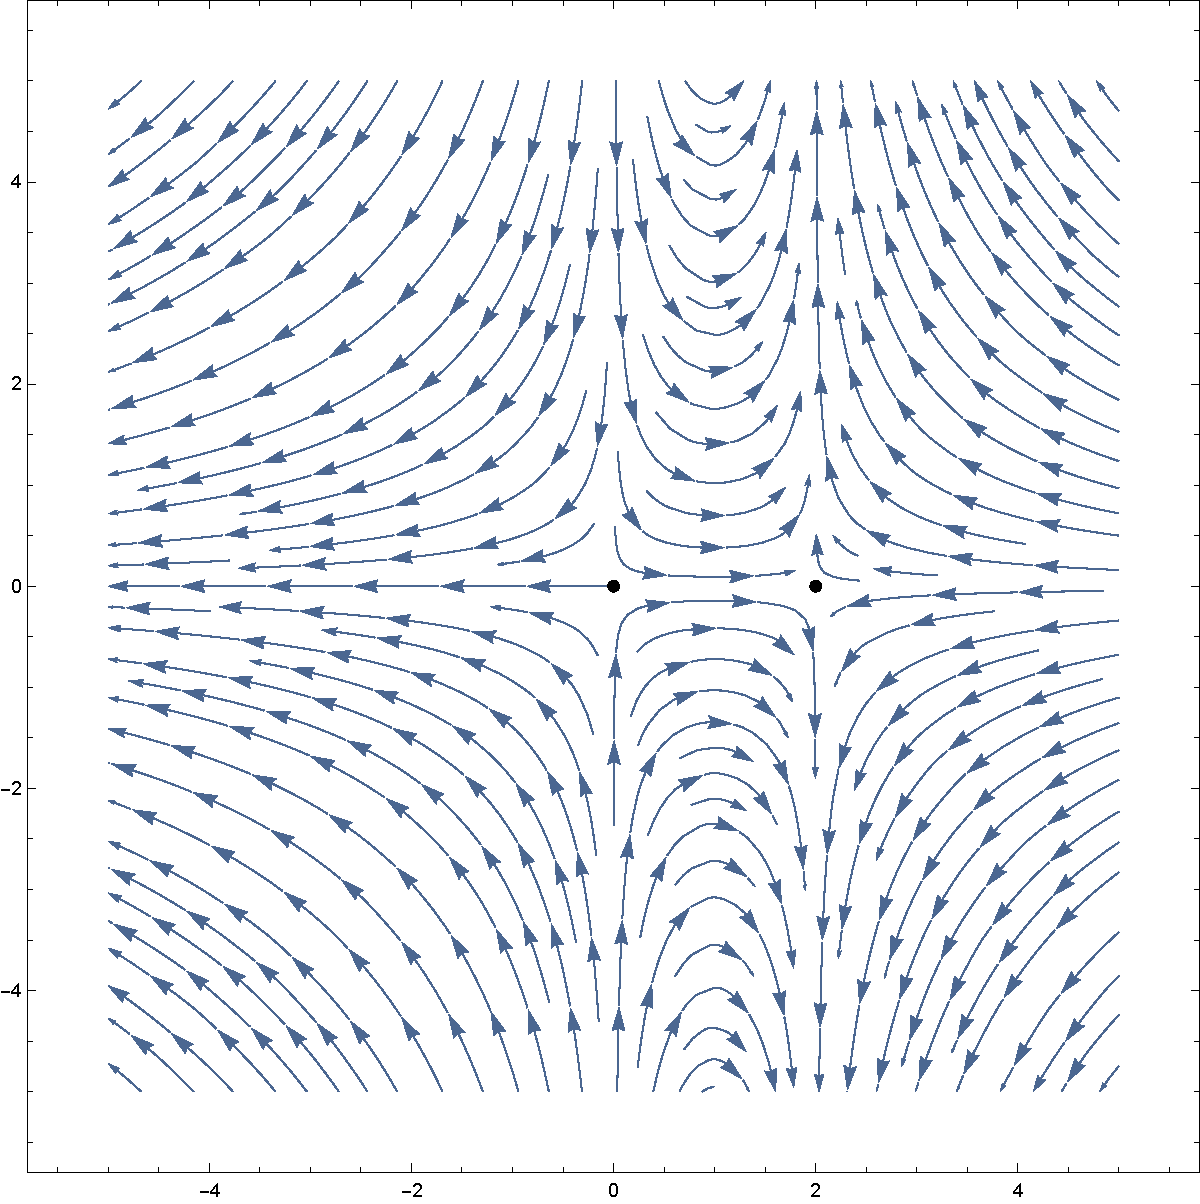
\includegraphics[width=0.8\textwidth]{figures/ex5_vecfComb.pdf}
        \caption{\gr{Διανυσματικό πεδίο συστήματος}}
        \label{fig:ex5_vecfComb}
    \end{figure}

    (β). Μία μη-εγκάρσια τομή στο απλό εκκρεμές είναι η τροχιά που ενώνει τα δύο
    σάγματα. Ελάχιστη μείωση της ενέργειας του εκκρεμούς θα μας πάει στην
    ευσταθή περιοχή, δηλαδή εντός της διαχωριστικής καμπύλης, και αντίστοιχα ελάχιστη
    αύξηση της ενέργειας στη ασταθή, δηλαδή πάνω από τη διαχωριστική καμπύλη.

    Αντίστοιχα είναι τα πράγματα στο σύστημα \tl{Duffing}. Εκεί έχουμε δύο
    περιοχές έλξης και διαχωριστική καμπύλη είναι ο περιστραμμένος κατά
    \( 90 \) αριθμός οκτώ.

    Το να φέρουμε τα συστήματα σε \enquote*{γενική θέση} μπορεί να σημαίνει να
    μεγαλώσουμε την περιοχή όπου τα συστήματα είναι ευσταθή. Ένας τρόπος όπως
    είδαμε είναι με την προσθήκη της απόσβεσης. Θέλουμε όμως να
    παραμείνουμε στην κατηγορία των Χαμιλτονιανών συστημάτων. Η συμπεριφορά των
    Χαμιλτονιανών συστημάτων, του εκκρεμούς και του \tl{Duffing}, θα παραμείνει
    ποιοτικά όπως την περιγράψαμε. Αυτό που μπορούμε να κάνουμε είναι να
    μεγαλώσουμε το χώρο της ευστάθειας. Για παράδειγμα μπορούμε να αλλάξουμε τη συχνότητα
    της ταλάντωσης του εκκρεμούς. Έστω δηλαδή ότι στη συνάρτηση δυναμικού
    όπου \( x \to 0.5x \), τότε θα μεγαλώνουμε το χώρο που είμαστε σε ευστάθεια.
    Αντίστοιχη λογική μπορούμε να ακολουθήσουμε στο σύστημα \tl{Duffing}.
\end{solution}
